% ss_setup.tex

% Setting up the board
\subsection{Setting up the board}
\label{sec:settinguptheboard}
Like most things in the Realm of Thin-Things, there is not much room for humour.
Therefore, the joker has no place in either Kingdom; remove all jokers from the deck.

The \textbf{Shuffle-Spires} board is set up using the Kings, Queens and Jacks (of all suits) to represent the four Spires and their three sections.
One could imagine the Spires stretching outward from the center.
Shuffle the rest of the deck, containing cards one-through-ten (Ace being nr. 1) from all suits, and place it in the middle of the board.
The Spires thusly create three different zones on the board, which will represent progression of the attacking Henchmen.

Each player chooses a King (a suit, rather), and places him-/herself next to the currently inhabited Spire.
Note that the player is not the owner of any specific Spire, but rather three parts that will change location during play.

The King of Hearts starts off with the title \textit{'The Thin-Things-Thin'}, to signify him being the current Ruler of the Realm of Thin-Things.
The title dictates when the Henchmen are moved further towards the center of the Spires.
This title may be given unto someone else during play, which will be explained in latter parts of this ruleset.

\begin{figure}[h!]
	\centering
	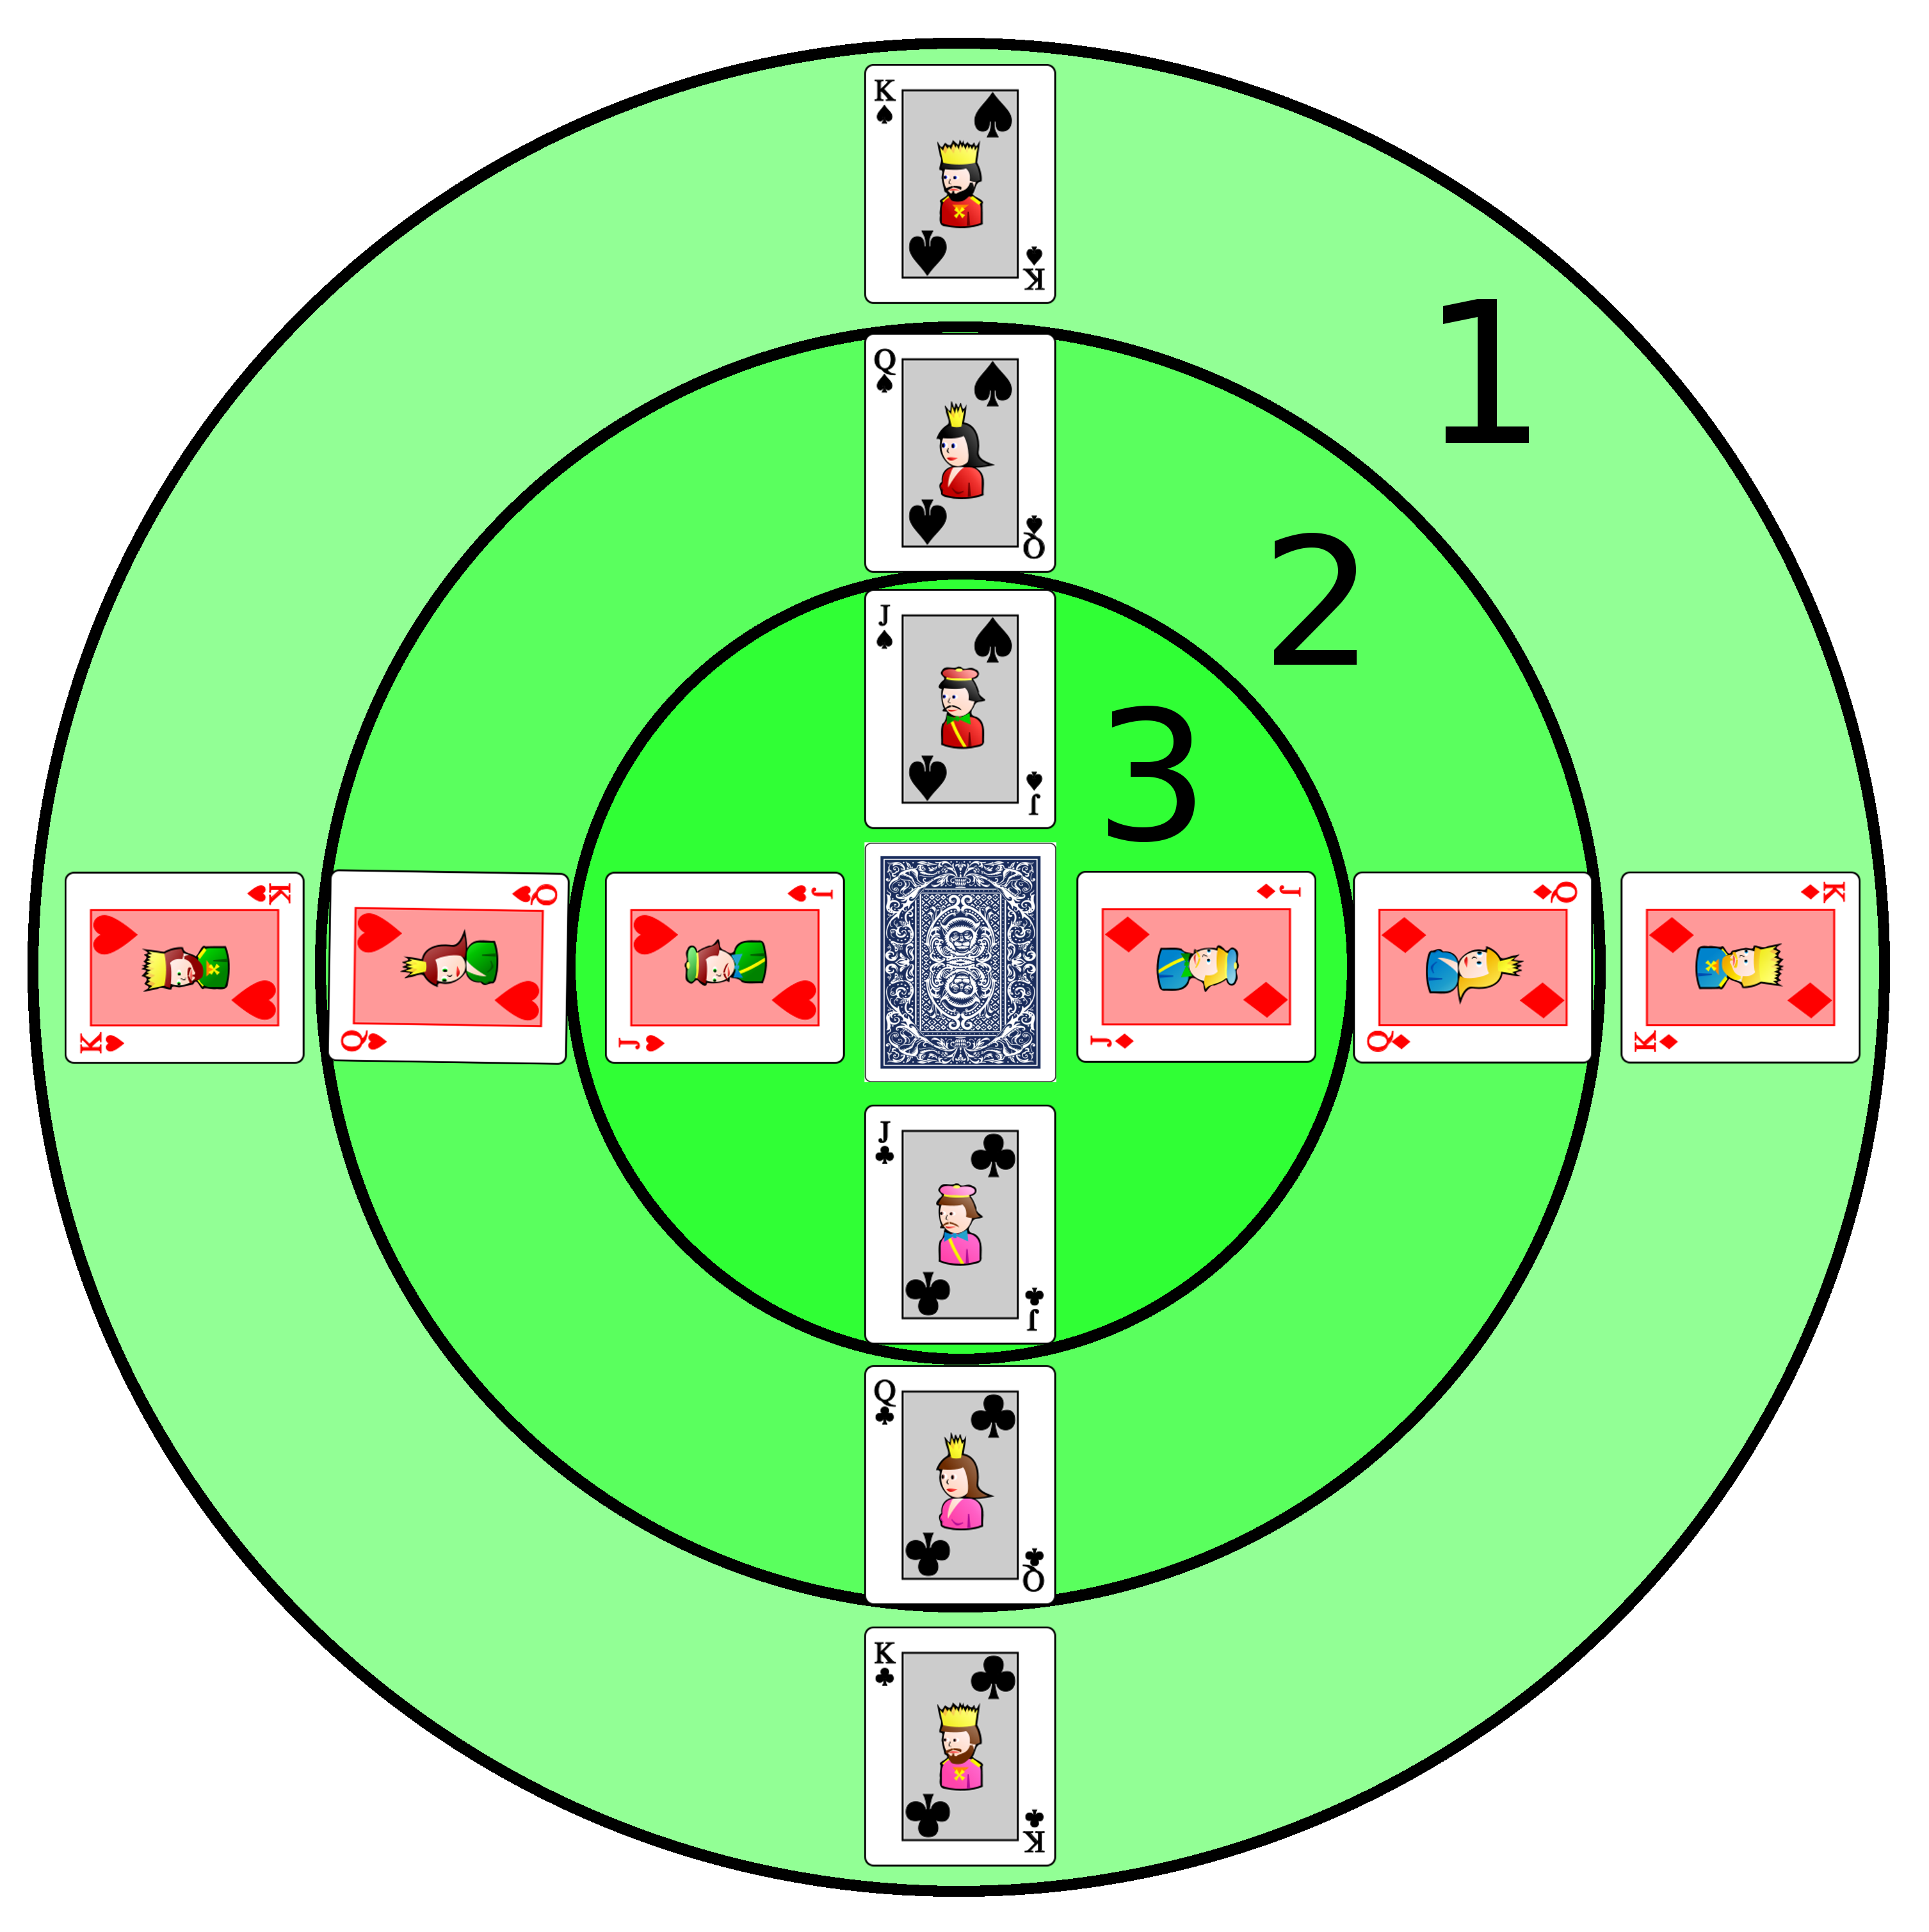
\includegraphics[width=\linewidth]{img/starting.png}
	\caption{Starting board and progression zones.}
	\label{fig:starting}
\end{figure}

\paragraph{Note}
Since the Spires may shuffle and swap during play, in this ruleset, \textit{'X's Spire'} will signify the Spire Player X's King currently resides in.
